\chapter{磁気強度による自己位置推定の開発}

\graphicspath{{figures/04}}


\section{はじめに}
\label{sec:kalman_filter}

\section{磁気センサのキャリブレーション}
\subsection{球面フィッティングによるオフセット値の算出と軸バイアスの補正}

\section{ガウス過程回帰による磁気地図構築}
\subsection{磁気強度の取得}
\subsection{ガウス過程回帰を用いた磁気地図構築}

\section{局所GPRを用いた大規模磁気地図作成}
\subsection{K-means法による観測データのクラスタリング}
\subsection{局所GPRを用いた磁気地図構築}

\section{磁気強度に基づく自己位置推定}

\section{LiDARと磁気強度に基づく自己位置推定の統合}

\section{実環境における自己位置推定実験}
\subsection{実験方法}
本研究では，実環境の屋内外と人混み環境の屋外において有効な位置推定手法であるかを評価するため，
開発した磁気強度に基づく自己位置推定と提案するLiDARと磁気を統合した自己位置推定の評価を行った．
実験は，調布市のショッピングセンタと大阪・関西万博の会場内で実施した．
はじめに，ロボットが地図作成のための経路と実験用の経路を走行し，磁気強度，オドメトリ，LiDARによる
点群情報，そして混雑時の万博ではichimillによるGNSSのデータをrosbagに記録した．
その後，rosbagから幾何地図及び磁気地図を作成した．
最後に，実験用のrosbagから位置推定精度の検証を行った．
ショッピングセンタや万博会場ではLiDAR MCLの結果を真値とし，
混雑時の万博会場ではGNSSデータを真値の軌跡として扱った．
特に，LiDAR MCL（ESS＝0.99）と比較して，LiDAR MCL，Mag MCL，LiDAR-Mag MCLの3手法を比較した．
各手法のESSの閾値は0.9，パーティクル数は500個とし，屋内地図のグリッドサイズは0.1[m]，
磁気地図および屋外地図のグリッドサイズは0.2[m]とした．

\subsection{実験結果}
% -----------------------------
% Table 1: Shopping Center
% -----------------------------
\begin{table}[H]
  \centering
  \caption{Localization Error Statistics (shopping center)}
  \label{tab:error_shopping}
  \renewcommand{\arraystretch}{1.2}
  \begin{tabular}{|l|c|c|c|c|}
    \hline
    sensor & mae [m] & rmse [m] & std [m] & max [m] \\
    \hline
    LiDAR & 0.13 & 0.15 & 0.09 & 0.43 \\
    Mag   & 0.21 & 0.23 & 0.11 & 0.52 \\
    LiDAR-Mag & 0.18 & 0.18 & 0.08 & 0.38 \\
    \hline
  \end{tabular}
\end{table}

% -----------------------------
% Table 2: Expo (Low Crowd)
% -----------------------------
\begin{table}[H]
  \centering
  \caption{Localization Error Statistics (Expo)}
  \label{tab:error_expo_low}
  \renewcommand{\arraystretch}{1.2}
  \begin{tabular}{|l|c|c|c|c|}
    \hline
    sensor & mae [m] & rmse [m] & std [m] & max [m] \\
    \hline
    LiDAR & 11.45 & 16.87 & 12.39 & 54.07 \\
    Mag   & 2.26 & 2.49  & 1.05  & 3.64 \\
    LiDAR-Mag & 0.78 & 1.29  & 1.02  & 4.14 \\
    \hline
  \end{tabular}
\end{table}

\begin{figure}[H]
  \centering
  % figures/sample.png を置くか、パスを差し替え
  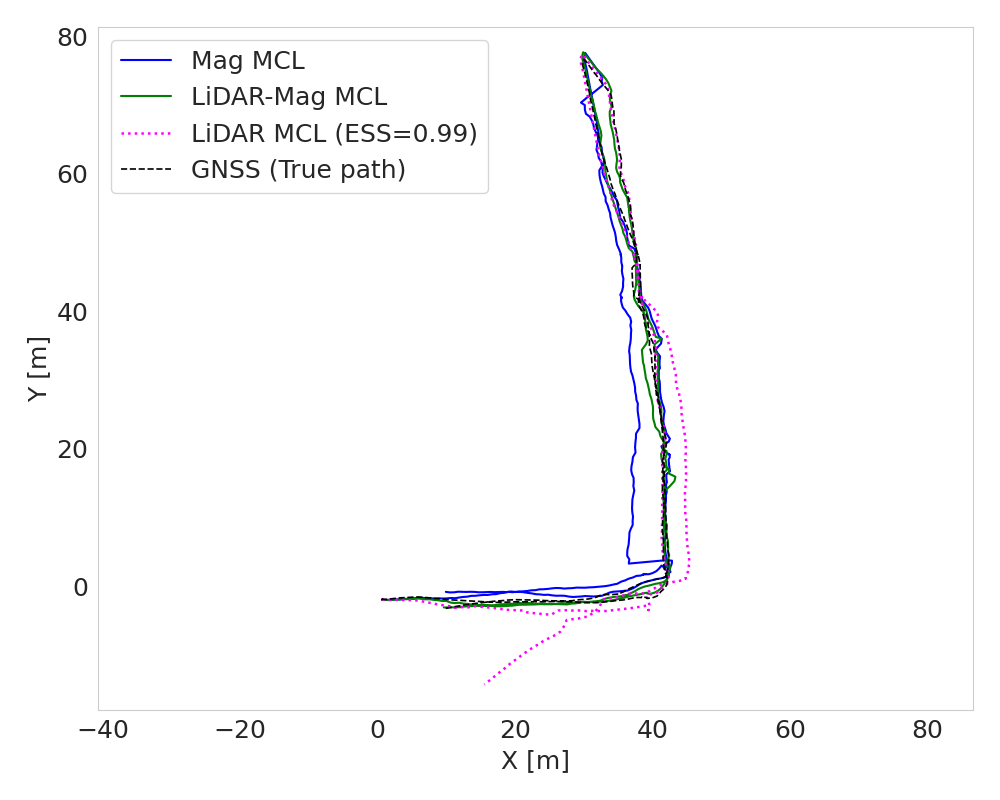
\includegraphics[width=0.3\columnwidth]{lidar_mag_plot.png}
  \caption{Robot trajectories estimated by Mag MCL, LiDAR-Mag MCL, LiDAR MCL (ESS = 0.99), and GNSS in the crowded Expo environment}
  \label{fig:sample}
\end{figure}

ショッピングセンタ及び万博会場実験結果を\cref{tab:error_shopping}，
\cref{tab:error_expo_low}に,
混雑時における万博会場の各位置推定ごとの軌跡を\cref{fig:sample}に示す．
\cref{tab:error_shopping}より磁気強度変化が大きいショッピングにおいては，Mag MCLが
LiDAR MCLの自己位置推定と同程度の位置推定精度を実現した．
Akaiらが報告した位置誤差0.8[m]以下を実環境で達成したことから，
今回開発した磁気による自己位置推定が実環境において有効であると示した．
また\cref{tab:error_expo_low}にから，
ESSが0.9のLiDAR MCLでは自己位置推定が破綻していることが確認できる．
一方で，Mag MCL及びLiDAR-Mag MCLでは若干の誤差が生じているものの，
安定した位置推定が実行できている．
さらに，\cref{fig:sample}に示す混雑時の万博会場の軌跡から，
ESS=0.99のLiDAR MCLでは自己位置推定が失敗しているのに対し，
Mag MCLおよびLiDAR-Mag MCLはGNSS軌跡に追従しており，
本手法が人混み環境においても有効であることを示した．
最後に，LiDAR-Mag MCLはMag MCLと比較してRMSEが小さいく，
GNSSの軌跡により近いことから精度が向上していることがわかる．
したがって異なるセンサ情報を統合することにより，
より高精度かつ安定した自己位置推定が可能であることを示した．

\section{考察}
実験結果から本研究で開発した磁気による自己位置推定および提案手法が実環境の屋内外および
人混み環境において有効であると示した．
一方で，ショッピングセンタに比べ万博会場のMag MCLの位置推定精度が低かった要因として，
\cref{fig:magmap_comparison}より今回作成した磁気地図が万博会場だと磁気強度の変化する箇所が
少ないため，ランドマークが少なく精度が低下したと推察できる．
また，ショッピングセンタの磁気地図構築時の磁気強度の変化幅が282.3[$\displaystyle \mu$T],
万博会場では106.9[$\displaystyle \mu$T]であり，万博会場の磁気強度の変動が小さいことが
精度低下の要因だと考える．
LiDAR-Mag MCLは，実環境において安定した自己位置推定ができており，
通常時や混雑時の万博会場においてもMag MCLよりも安定した挙動である．
これは，LiDARと磁気情報を組み合わせることで尤度分布が鋭くなり，パーティクルごとの尤度差が顕著になり収束しやすくなったと考察できる．
また，磁気強度に変化のある領域では，パーティクルが局所的に収束する．
よって，LiDARが安定的に観測できる構造物を識別しやすくなる．
さらに，ロボットが人混みを抜けてランドマークが観測できた際には，
真値付近に存在するパーティクルの尤度が高くなることで，
人混み環境においても自己位置推定精度が向上したと考察する．
次に，今後LiDARの自己位置推定が失敗したときの切り替え手法に向けて考察する．
\cref{tab:lidar_env_comparison}は，LiDAR MCLのESS，尤度平均，
およびパーティクルの広がりを示す指標$\sqrt{\sigma_x^2+\sigma_y^2}$の平均値
をそれぞれ算出し，各環境ごとに示している．
\cref{tab:lidar_ess99}は，LiDAR MCL (ESS=0.99)が位置推定に失敗した混雑時の万博のデータを示している．
\cref{tab:lidar_env_comparison}から，位置推定に成功したショッピングセンタと比較して，
万博会場では尤度平均が低下し，パーティクルの広がりも大きいことが確認できる．
これら2つの指標は，LiDAR MCLの位置推定失敗を検知する有効な指標となる．
一方で，\cref{tab:lidar_ess99}では，パーティクルの広がりは小さい場合でも
尤度が低下する場合も存在するため，これらの指標だけでは誤検知の可能性がある．
そのため磁気や提案手法の自己位置推定との比較や
パーティクル分布から算出される誤差楕円内に
LiDAR MCLの推定結果が含まれるかどうかの指標を併用することで，
失敗検知が可能になると考える．


\begin{figure}[H]
  \centering
  \begin{subfigure}[t]{0.25\columnwidth}
    \centering
    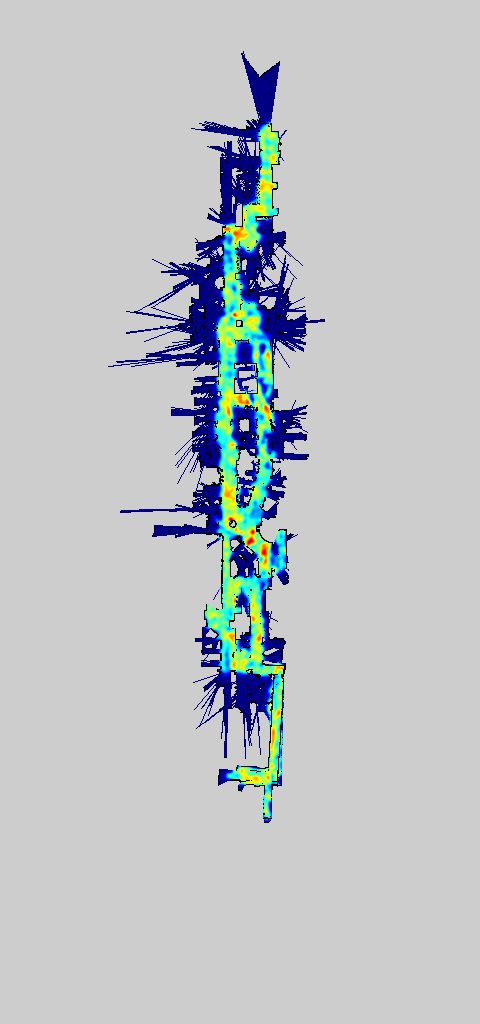
\includegraphics[width=\linewidth]{geomag_map.png}
    \caption{Shopping center}
    \label{fig:imu_accel}
  \end{subfigure}
  \hfill
  \begin{subfigure}[H]{0.3\columnwidth}
    \centering
    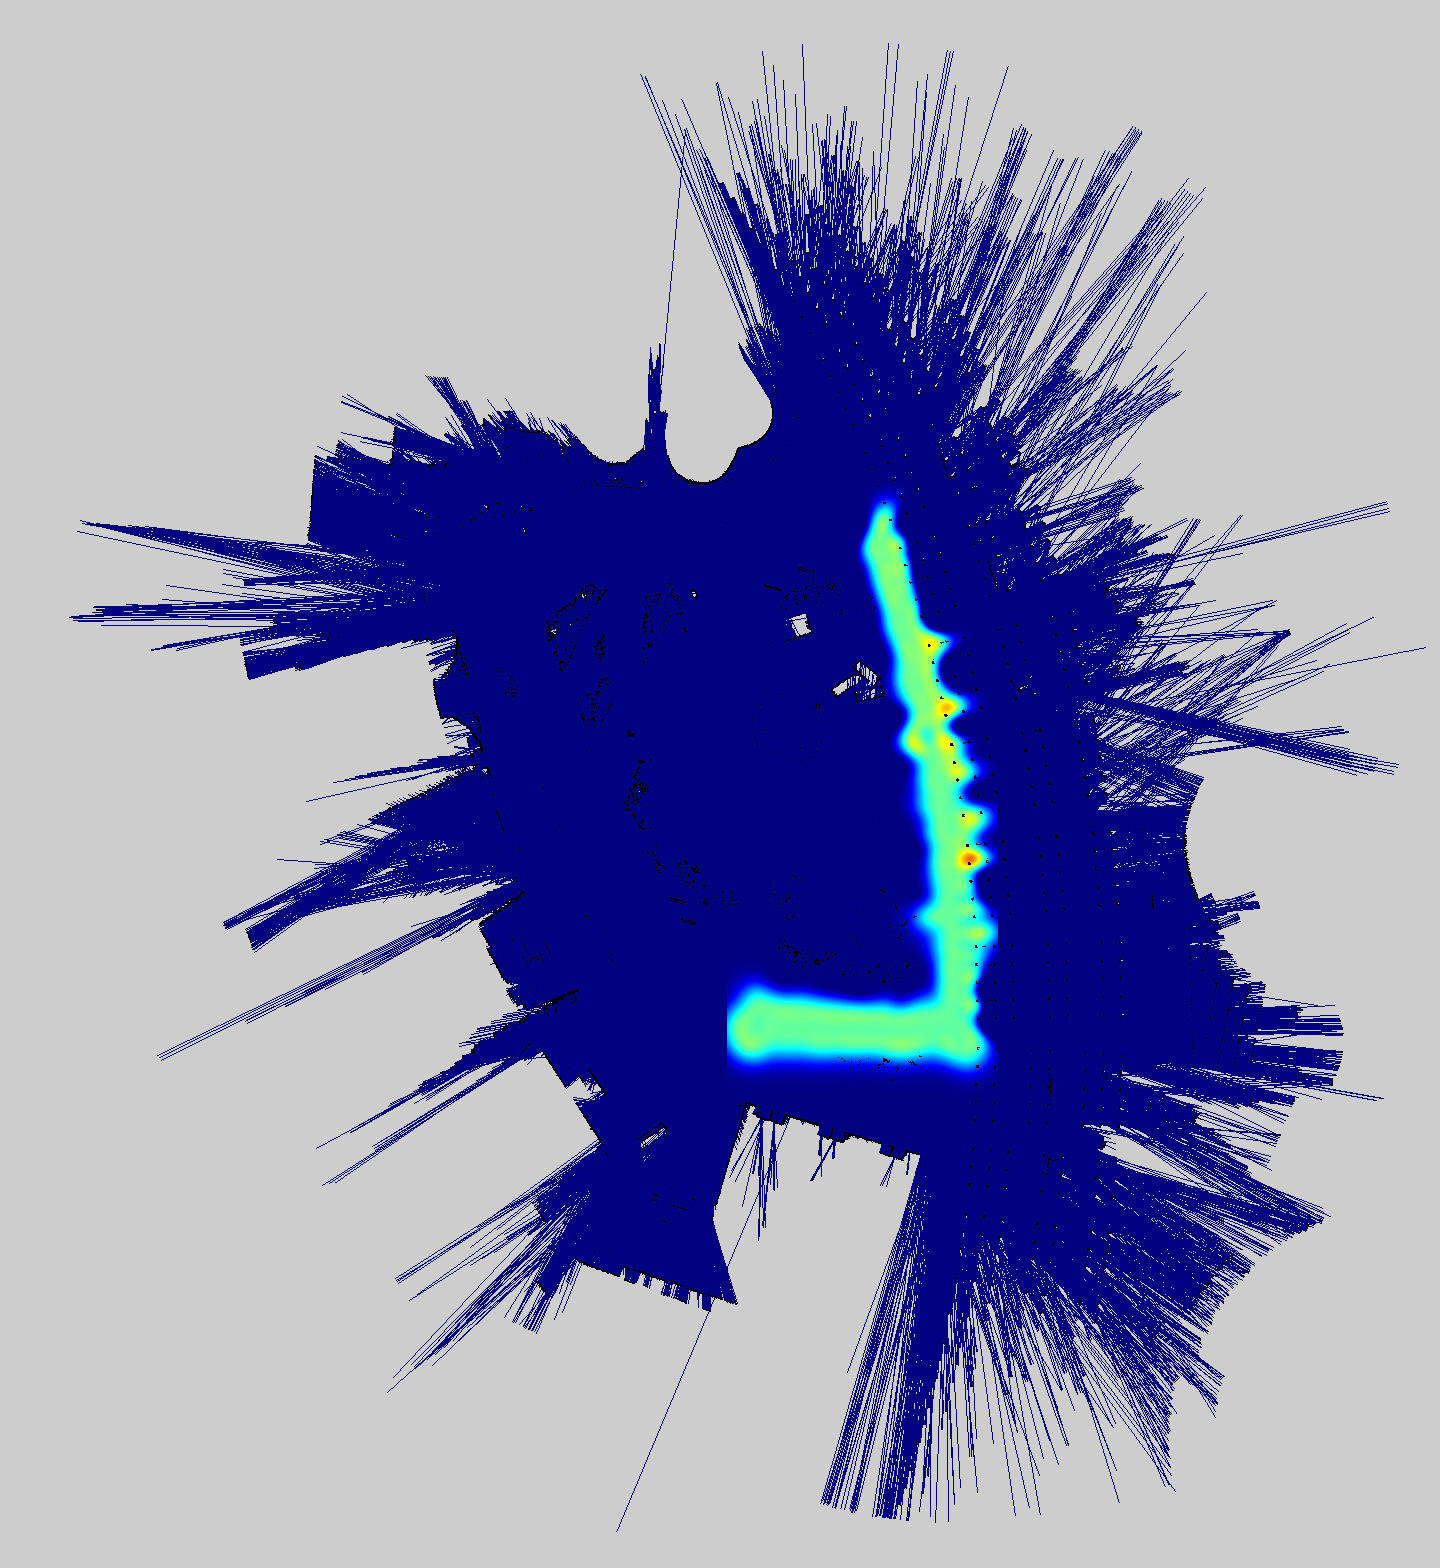
\includegraphics[width=\linewidth]{geomag_map.jpg}
    \caption{Expo site}
    \label{fig:imu_gyro}
  \end{subfigure}
  \caption{Comparison between the magnetic maps of the shopping center and the Expo site.}
  \label{fig:magmap_comparison}
\end{figure}

\begin{table}[t]
  \centering
  \caption{Mean values of ESS, likelihood, and position variance ($\sqrt{\sigma_x^2+\sigma_y^2}$) for LiDAR MCL under different environments}
  \label{tab:lidar_env_comparison}
  \begin{tabular}{|c|c|c|c|}
    \hline
    environment & ESS & likelihood & position variance [m] \\
    \hline
    Shopping Center & 0.84 & 0.56 & 0.92 \\
    Expo & 0.84 & 0.08 & 15.93 \\
    Expo (Crowded) & 0.95 & 0.09 & 13.97 \\
    \hline
  \end{tabular}
\end{table}
\begin{table}[t]
  \centering
  \caption{Mean values of ESS, likelihood, and position variance for LiDAR MCL (ESS = 0.99) in the crowded Expo environment}
  \label{tab:lidar_ess99}
  \begin{tabular}{|c|c|c|c|}
    \hline
    environment & ESS & likelihood & position variance [m] \\
    \hline
    Expo (Crowded) & 0.98 & 0.11 & 0.50 \\
    \hline
  \end{tabular}
\end{table}

\section{おわりに}
本稿では，磁気強度を用いた不可視地図に基づく自己位置推定および
磁気とLiDARを統合した自己位置推定手法を提案し，実環境の屋内外および
人混み環境での自己位置推定実験を行った．
結果として，磁気や提案手法による位置推定は，実環境およびLiDARの位置推定が失敗するほど
の人混み環境においても安定した自己位置推定が可能であると判明した．
今後は，LiDARの自己位置推定の失敗を検知し，他の位置推定手法に切り替えるためのシステム
の構築を目指す．